%%%%%%%%%%%%%%%%%%%%%%%%%%%%%%%%%%%%%%%%%
% Arsclassica Article
% LaTeX Template
% Version 1.1 (1/8/17)
%
% This template has been downloaded from:
% http://www.LaTeXTemplates.com
%
% Original author:
% Lorenzo Pantieri (http://www.lorenzopantieri.net) with extensive modifications by:
% Vel (vel@latextemplates.com)
%
% License:
% CC BY-NC-SA 3.0 (http://creativecommons.org/licenses/by-nc-sa/3.0/)
%
%%%%%%%%%%%%%%%%%%%%%%%%%%%%%%%%%%%%%%%%%

%----------------------------------------------------------------------------------------
%	PACKAGES AND OTHER DOCUMENT CONFIGURATIONS
%----------------------------------------------------------------------------------------

\documentclass[
10pt, % Main document font size
a4paper, % Paper type, use 'letterpaper' for US Letter paper
oneside, % One page layout (no page indentation)
%twoside, % Two page layout (page indentation for binding and different headers)
headinclude,footinclude, % Extra spacing for the header and footer
BCOR5mm, % Binding correction
]{scrartcl}
\usepackage{graphicx}

%%%%%%%%%%%%%%%%%%%%%%%%%%%%%%%%%%%%%%%%%
% Arsclassica Article
% Structure Specification File
%
% This file has been downloaded from:
% http://www.LaTeXTemplates.com
%
% Original author:
% Lorenzo Pantieri (http://www.lorenzopantieri.net) with extensive modifications by:
% Vel (vel@latextemplates.com)
%
% License:
% CC BY-NC-SA 3.0 (http://creativecommons.org/licenses/by-nc-sa/3.0/)
%
%%%%%%%%%%%%%%%%%%%%%%%%%%%%%%%%%%%%%%%%%

%----------------------------------------------------------------------------------------
%	REQUIRED PACKAGES
%----------------------------------------------------------------------------------------

\usepackage[
nochapters, % Turn off chapters since this is an article        
beramono, % Use the Bera Mono font for monospaced text (\texttt)
eulermath,% Use the Euler font for mathematics
pdfspacing, % Makes use of pdftex’ letter spacing capabilities via the microtype package
dottedtoc % Dotted lines leading to the page numbers in the table of contents
]{classicthesis} % The layout is based on the Classic Thesis style

\usepackage{arsclassica} % Modifies the Classic Thesis package

\usepackage[T1]{fontenc} % Use 8-bit encoding that has 256 glyphs

\usepackage[utf8]{inputenc} % Required for including letters with accents

\usepackage{graphicx} % Required for including images
\graphicspath{{Figures/}} % Set the default folder for images

\usepackage{enumitem} % Required for manipulating the whitespace between and within lists

\usepackage{lipsum} % Used for inserting dummy 'Lorem ipsum' text into the template

\usepackage{subfig} % Required for creating figures with multiple parts (subfigures)

\usepackage{amsmath,amssymb,amsthm} % For including math equations, theorems, symbols, etc

\usepackage{varioref} % More descriptive referencing

%----------------------------------------------------------------------------------------
%	THEOREM STYLES
%---------------------------------------------------------------------------------------

\theoremstyle{definition} % Define theorem styles here based on the definition style (used for definitions and examples)
\newtheorem{definition}{Definition}

\theoremstyle{plain} % Define theorem styles here based on the plain style (used for theorems, lemmas, propositions)
\newtheorem{theorem}{Theorem}

\theoremstyle{remark} % Define theorem styles here based on the remark style (used for remarks and notes)

%----------------------------------------------------------------------------------------
%	HYPERLINKS
%---------------------------------------------------------------------------------------

\hypersetup{
%draft, % Uncomment to remove all links (useful for printing in black and white)
colorlinks=true, breaklinks=true, bookmarks=true,bookmarksnumbered,
urlcolor=webbrown, linkcolor=RoyalBlue, citecolor=webgreen, % Link colors
pdftitle={}, % PDF title
pdfauthor={\textcopyright}, % PDF Author
pdfsubject={}, % PDF Subject
pdfkeywords={}, % PDF Keywords
pdfcreator={pdfLaTeX}, % PDF Creator
pdfproducer={LaTeX with hyperref and ClassicThesis} % PDF producer
} % Include the structure.tex file which specified the document structure and layout

\hyphenation{Fortran hy-phen-ation} % Specify custom hyphenation points in words with dashes where you would like hyphenation to occur, or alternatively, don't put any dashes in a word to stop hyphenation altogether

%----------------------------------------------------------------------------------------
%	TITLE AND AUTHOR(S)
%----------------------------------------------------------------------------------------

\title{\normalfont\spacedallcaps{Herramienta para detección de enfermedades de salud mental}} % The article title

%\subtitle{Subtitle} % Uncomment to display a subtitle

\author{\spacedlowsmallcaps{José Luis Leiva, Eduardo García Maleta, Jesús Aldair Alfonso}} % The article author(s) - author affiliations need to be specified in the AUTHOR AFFILIATIONS block

\date{} % An optional date to appear under the author(s)

%----------------------------------------------------------------------------------------

\begin{document}

%----------------------------------------------------------------------------------------
%	HEADERS
%----------------------------------------------------------------------------------------

\renewcommand{\sectionmark}[1]{\markright{\spacedlowsmallcaps{#1}}} % The header for all pages (oneside) or for even pages (twoside)
%\renewcommand{\subsectionmark}[1]{\markright{\thesubsection~#1}} % Uncomment when using the twoside option - this modifies the header on odd pages
\lehead{\mbox{\llap{\small\thepage\kern1em\color{halfgray} \vline}\color{halfgray}\hspace{0.5em}\rightmark\hfil}} % The header style

\pagestyle{scrheadings} % Enable the headers specified in this block

%----------------------------------------------------------------------------------------
%	TABLE OF CONTENTS & LISTS OF FIGURES AND TABLES
%----------------------------------------------------------------------------------------

\maketitle % Print the title/author/date block

\setcounter{tocdepth}{2} % Set the depth of the table of contents to show sections and subsections only

%\tableofcontents % Print the table of contents

% \listoffigures % Print the list of figures

% \listoftables % Print the list of tables

%----------------------------------------------------------------------------------------
%	ABSTRACT
%----------------------------------------------------------------------------------------

% \section*{Abstract} % This section will not appear in the table of contents due to the star (\section*)

% \lipsum[1] % Dummy text

% %----------------------------------------------------------------------------------------
% %	AUTHOR AFFILIATIONS
% %----------------------------------------------------------------------------------------

% \let\thefootnote\relax\footnotetext{* \textit{Department of Biology, University of Examples, London, United Kingdom}}

% \let\thefootnote\relax\footnotetext{\textsuperscript{1} \textit{Department of Chemistry, University of Examples, London, United Kingdom}}

%----------------------------------------------------------------------------------------

\newpage % Start the article content on the second page, remove this if you have a longer abstract that goes onto the second page

%----------------------------------------------------------------------------------------
%	Corrupcion
%----------------------------------------------------------------------------------------
\begin{center}
\textbf{Abstract}
\end{center}    
\begin{abstract}
Este artículo presenta un estudio comprensivo sobre el análisis de enfermedades de salud mental en redes sociales utilizando técnicas de aprendizaje automático.
Exploramos diversas metodologías para la extracción de características, incluyendo el uso del léxico Empath para cuantificar los tonos emocionales
en contenido generado por usuarios. En nuestro análisis se emplea herramientas de aprendizaje automático, tanto supervisado como no supervisado; 
evaluando el rendimiento de diferentes modelos a través de validación cruzada estratificada, proporcionando información sobre sus capacidades predictivas. Los modelos utilizados en 
este trabajo fueron K-Means y Redes Neuronales. 
\end{abstract}


\section*{Palabras Clave :} Análisis de Sentimientos, Clasificación de Enfermedades de Salud Mendal, Aprendizaje Automático, Redes
Sociales, Extracción de Características, KMeans, Redes Neuronales.

\tableofcontents

\section{Estado del Arte}

1. \textbf{Sentiment Analysis of Mental Health Using K-Nearest Neighbors on Social Media Twitter (2022)} \\
   \textbf{Modelos}: KNNs, SVM y Árboles de Decisión. \\
   \textbf{Método}: Procesamiento de datos utilizando KNNs, comparando el algoritmo de clasificación de Máquinas de Soporte Vectorial y el procesamiento de datos de Árboles de Decisión utilizando herramientas de "RapidMiner". \\
   \textbf{Resultados}: Separando la data en un ratio de 70:30 y usando k=5, la eficacia fue de 58.39\%. \\
   \textbf{Dataset}: Revisiones de la comunidad con el keyword "Mental Health".

2. \textbf{Depression Detection from Social Network Data Using Machine Learning Techniques (2018)} \\
   \textbf{Modelos}: SVM, Árboles de Decisión, Clasificadores por Conjuntos y KNNs. \\
   \textbf{Método}: Análisis de depresión usando cuatro modelos sobre un conjunto de atributos como el "proceso emocional", el "proceso temporal" y el "estilo lingüístico". \\
   \textbf{Resultados}: Decision Trees y SVM tienen una eficacia entre el 70\% y 73\%; KNNs y Ensemble Classifiers tienen una eficacia entre el 60\% y 64\%. \\
   \textbf{Dataset}: Comentarios de usuarios en Facebook.

3. \textbf{Depression Detection by Analyzing Social Media Posts of Users (2019)} \\
   \textbf{Modelos}: SVM y Naive Bayes. \\
   \textbf{Método}: Clasificación de oraciones tokenizadas con Naive Bayes. \\
   \textbf{Resultados}: Eficacia del 74\%. \\
   \textbf{Dataset}: Utilización de un diccionario de sentimientos y colección de tweets obtenidos con "BeautifulSoup".

4. \textbf{MM-EMOG: Multi-Label Emotion Graph Representation for Mental Health Classification on Social Media (2024)} \\
   \textbf{Modelos}: TextGCN, MM-EMOG (TextGCN adaptado); comparado con BERT, RoBERTa, MentalBERT y MentalRoBERTa. \\
   \textbf{Método}: Uso de Redes Neuronales de Convolución Gráfica para representación emocional multietiqueta. \\
   \textbf{Resultados}: Eficacia entre 67.5\% y 71.9\% en TwitSuicide; entre 70.3\% y 73\% en CSSRS; entre 76\% y 78\% en Depression. \\
   \textbf{Dataset}: TwitSuicide, CSSRS.

5. \textbf{Towards Interpretable Mental Health Analysis with Large Language Models (2023)} \\
   \textbf{Modelos}: Múltiples LLMs como LLaMa, InstructGPT-3 y ChatGPT; comparado con BERT, RoBERTa, MentalBERT, MentalRoBERTa, CNN, GRU, BiLSTM\_Att y fastText. \\
   \textbf{Método}: Empleo de LLMs para el análisis emocional mediante estrategias de prompting. \\
   \textbf{Resultados}: En Zero-shot, ChatGPT supera a LLaMa e InstructGPT-3 en todos los datasets; en el dataset DR consigue un recall del 82.8\% y un F1-score del 82.4\%. En Emotion-enhanced CoT, ChatGPT logra un recall del 85.7\% y un F1-score del 84.2\% en el dataset DR; en el resto de datasets supera su performance respectivo en Zero-shot. \\
   \textbf{Dataset}: Dreaddit, Depression\_Reddit, CLPsych15, T-SID, SAD y CAMS.
   
\section{Introducción}

En la última década, el uso de redes sociales ha crecido exponencialmente, convirtiéndose en una plataforma fundamental 
para la expresión personal y la interacción social. Este fenómeno ha generado un vasto volumen de datos que pueden ser analizados 
para obtener información valiosa sobre diversos aspectos de la vida cotidiana, incluida la salud mental. La clasificación de enfermedades 
de salud mental a partir de comentarios en redes sociales representa un desafío significativo, dado que los datos son inherentemente ruidosos y subjetivos.

El presente trabajo se centra en la aplicación de técnicas de aprendizaje automático para abordar este problema. 
A diferencia de estudios previos que han predominado en el uso de enfoques de aprendizaje supervisado, como Máquinas de Vectores de Soporte (SVM), 
Árboles de Decisión y Naive Bayes, nuestro enfoque inicial se basa en el aprendizaje no supervisado. Esta elección se fundamenta en la escasez de investigaciones 
que exploren esta metodología en el contexto específico del análisis de comentarios en redes sociales relacionados con la salud mental. Al emplear técnicas no supervisadas, 
buscamos evaluar su eficacia para identificar patrones y agrupaciones en los datos sin la necesidad de etiquetas predefinidas.

Posteriormente, complementamos nuestro análisis con un enfoque supervisado utilizando redes neuronales. A pesar de su creciente popularidad en el campo del aprendizaje automático, 
encontramos que su aplicación específica a la clasificación de enfermedades mentales a partir de datos extraídos de redes sociales es limitada en la literatura existente. 
 
A través de este trabajo, esperamos proporcionar una visión integral sobre cómo algunas de las herramientas de aprendizaje automático pueden ser utilizadas para abordar problemas complejos en el ámbito de la salud mental, abriendo nuevas vías para futuras investigaciones y aplicaciones prácticas.

\section{Desarrollo}

\subsection{Datos y Procesamiento}

Los datos utilizados en este estudio provienen de un conjunto de datos disponible en línea, el cual está catalogado en siete clases diferentes: 
Ansiedad, Depresión, Normal, Suicida, Estrés, Bipolar y Desorden de la Personalidad. Cada entrada del conjunto de datos está estructurada en dos columnas: 
una que contiene el texto y otra que proporciona la etiqueta correspondiente que describe la patología asociada al texto.

El primer paso en nuestro proceso de análisis fue la limpieza de los datos. Esto incluyó la eliminación de valores NaN (Not a Number) para asegurar la integridad del conjunto de datos. 

Una vez limpiados los datos, utilizamos \textbf{Empath}, que es una herramienta diseñada para caracterizar y cuantificar aspectos psicológicos del texto. 
Esta nos permitió extraer características relevantes que reflejan el contenido emocional y psicológico de los comentarios, facilitando así un análisis más profundo.

Posteriormente, aplicamos una matriz de correlación para identificar y eliminar datos redundantes dentro de nuestro conjunto. 
Esta técnica es esencial para reducir la dimensionalidad del dataset y mejorar la eficiencia del modelo, al eliminar características que no aportan información adicional o que están altamente correlacionadas con otras. 
Al final de este proceso, obtuvimos un conjunto de datos más limpio y representativo, listo para ser utilizado en nuestros modelos de aprendizaje automático.


\subsection{Enfoque No Supervisado Utilizando KMeans}

Para abordar la clasificación de enfermedades de salud mental, como primer enfoque utilizando el algoritmo KMeans. Este algoritmo es ampliamente reconocido por su capacidad para agrupar datos en clústeres basados en similitudes, 
y en nuestro caso, se le indicó que clusterizara los datos en siete clases, alineándose con las categorías del conjunto de datos original.

Sin embargo, los resultados obtenidos no fueron satisfactorios. Al analizar la distribución de los clústeres generados, observamos que una de las clases contenía únicamente dos elementos, mientras que otra clase agrupaba 99 elementos. 
Dada la naturaleza del conjunto de datos, que cuenta con miles de entradas por clase, esta distribución indica un desempeño deficiente del modelo.

La presencia de un clúster con tan pocos elementos sugiere que el algoritmo no pudo identificar patrones significativos dentro de los datos para esa clase específica. Asimismo, la clase con 99 elementos podría estar representando una agrupación inadecuada,
lo que implica que el modelo no logró capturar la complejidad del conjunto de datos.

En conclusión, estos resultados nos llevan a la reflexión sobre la idoneidad del enfoque no supervisado en este contexto particular. A pesar de las expectativas iniciales, los resultados obtenidos no cumplen con los estándares necesarios para 
una clasificación efectiva y nos motivan a explorar enfoques alternativos.

\subsection{Enfoque supervisado}

\textbf{Redes Neuronles}\\

Este método fue aplicado a los datos que ya habían sido caracterizados previamente, con el objetivo de clasificar las enfermedades de salud mental en las siete categorías definidas en nuestro conjunto de datos.

A pesar de las expectativas iniciales, los resultados obtenidos no fueron satisfactorios. La precisión alcanzada fue del 14.85\%, un valor que claramente no cumple con los estándares necesarios para una clasificación efectiva. 
Este bajo rendimiento sugiere que el modelo no logró aprender patrones significativos a partir de los datos caracterizados, lo que podría deberse a varios factores.

Entre las posibles razones para este resultado se encuentran la complejidad inherente del problema, la arquitectura y parámetros de la red neuronal. La baja precisión indica que el modelo podría estar sobreajustado o subajustado, 
lo que resalta la necesidad de realizar un análisis más profundo y ajustes en el proceso de entrenamiento.

En resumen, aunque el uso de redes neuronales es prometedor en el campo del aprendizaje automático, los resultados obtenidos en este caso particular nos llevan a reconsiderar y optimizar nuestro enfoque para mejorar la eficacia en la clasificación de enfermedades de salud mental.\\


\textbf{Redes Neuronales Convolucionales}\\

Para implementar un enfoque más avanzado, utilizamos redes neuronales convolucionales (CNN), las cuales son especialmente efectivas para aprender patrones en datos estructurados en forma de matrices, 
como es el caso de los textos transformados en imágenes. Dado que las CNN operan sobre datos bidimensionales, realizamos una nueva transformación a nuestros datos, convirtiéndolos en matrices adecuadas 
para este tipo de red.

Nuestra estrategia incluyó dos enfoques diferentes. En primer lugar, entrenamos el modelo utilizando los datos originales caracterizados, que fueron transformados en matrices de 128x194. 
En segundo lugar, aplicamos el mismo procedimiento a los datos resultantes del análisis de KMeans (teniendo que eliminar 2 clases debido a la falta de ekementos para crear las matrices), 
que fueron organizados en matrices de 128x172. En ambos casos, seleccionamos 128 datos aleatorios de cada clase para asegurar una representación equilibrada durante el entrenamiento.

Los resultados obtenidos fueron modestos. En el caso de los datos originales caracterizados, logramos una precisión del 17.56\%, mientras que al utilizar los datos derivados del KMeans, 
la precisión se redujo a 16.37\%. Estos resultados indican que, aunque las redes neuronales convolucionales tienen un gran potencial para la clasificación de patrones complejos, en este estudio 
no lograron alcanzar un rendimiento satisfactorio. 

Este desempeño sugiere que es necesario realizar ajustes adicionales en la arquitectura de la red o en el preprocesamiento de los datos para mejorar la capacidad del modelo para generalizar y clasificar 
correctamente las distintas patologías asociadas a los comentarios en redes sociales.\\



Para entrenar todos los modelos, se utilizó la validación cruzada, una técnica que permite evaluar la capacidad de generalizacón del modelo al dividir el conjunto de datos en múltiples subconjuntos y entrenar el modelo 
en diferentes combinaciones. Esto ayuda a mitigar el riesgo de sobreajuste y proporciona una estimación más robusta del rendimiento del modelo.
% A statement requiring citation \cite{Figueredo:2009dg}.

\section{Conclusiones}

El presente estudio ha explorado la clasificación de enfermedades de salud mental utilizando técnicas de aprendizaje automático, específicamente a través de enfoques no supervisados y supervisados. 
A pesar de las expectativas iniciales, los resultados obtenidos han evidenciado limitaciones significativas en ambos enfoques.

En el caso del aprendizaje no supervisado, el uso del algoritmo KMeans no logró proporcionar resultados satisfactorios. La distribución desigual de los clústeres, con algunas 
clases conteniendo muy pocos elementos, sugiere que este enfoque no fue adecuado para capturar la complejidad del conjunto de datos. Esto pone de manifiesto la necesidad de considerar otras 
metodologías o ajustes en el preprocesamiento de los datos.

Por otro lado, el uso de redes neuronales, incluyendo redes neuronales convolucionales como técnica de aprendizaje supervisado, también presentó desafíos. 
A pesar de realizar transformaciones adecuadas a los datos y aplicar validación cruzada, las precisiones alcanzadas (14.85\%, 17.56\% y 16.37\% para los datos originales y 
los derivados del KMeans, respectivamente) indican que los modelos no lograron aprender patrones significativos. Esto resalta la importancia de una selección cuidadosa de características y una 
arquitectura adecuada para mejorar el rendimiento del modelo.

En conclusión, aunque las herramientas de aprendizaje automático ofrecen un gran potencial para abordar problemas complejos en el ámbito de la salud mental, este estudio ha demostrado que se requieren enfoques más refinados 
y experimentales para lograr resultados efectivos. Futuros trabajos podrían beneficiarse al explorar diferentes arquitecturas de redes neuronales, así como técnicas avanzadas de preprocesamiento y selección de características, 
con el fin de mejorar la clasificación y contribuir a una mejor comprensión y tratamiento de las enfermedades mentales a través del análisis de datos extraídos de redes sociales.

\section{Anexos}


\begin{figure}[tb]
\centering 
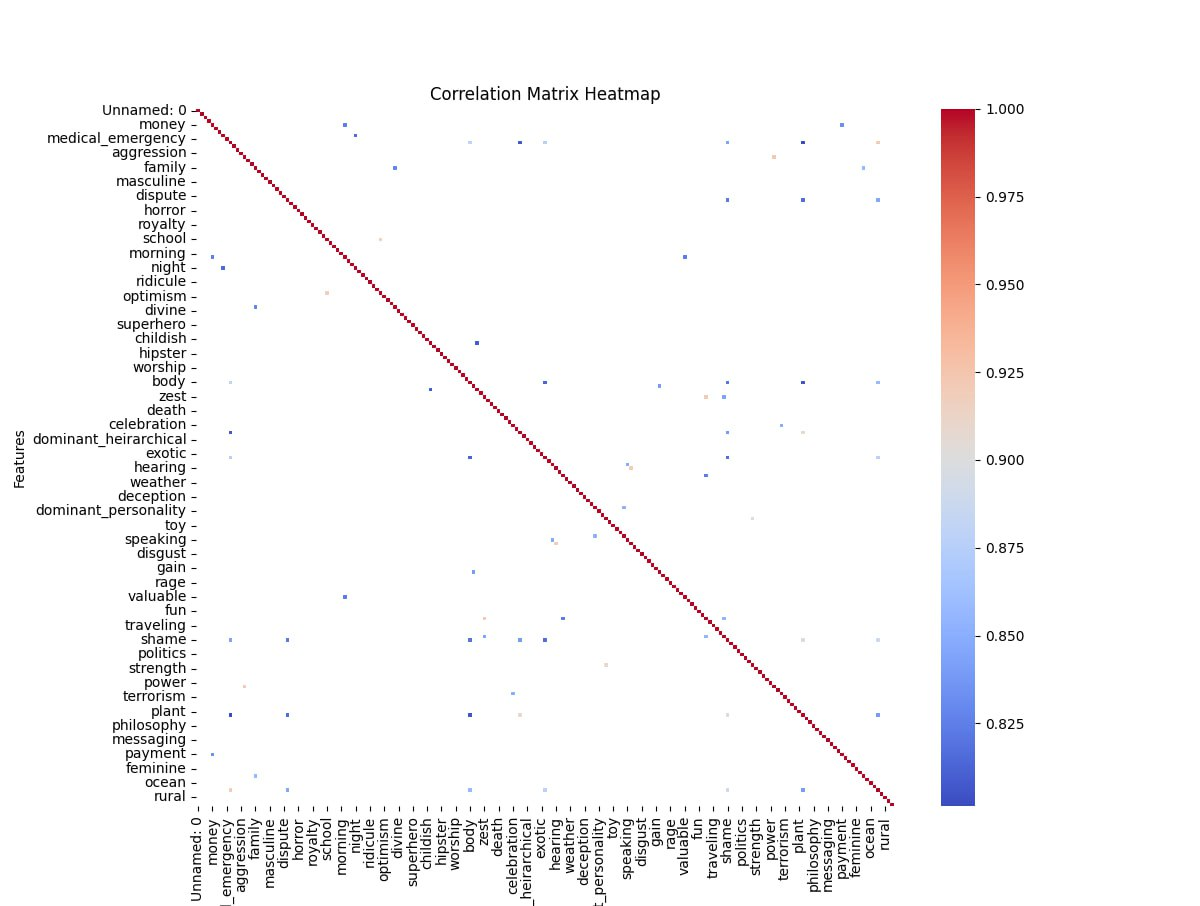
\includegraphics[width=1.3\columnwidth]{matrix} 
\caption[]{Matriz de correlación.} % The text in the square bracket is the caption for the list of figures while the text in the curly brackets is the figure caption
\label{fig:gallery} 
\end{figure}

\begin{figure}[tb]
\centering 
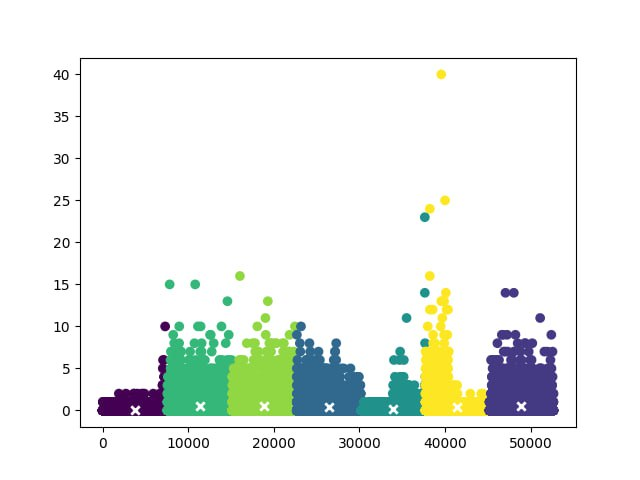
\includegraphics{kmeans} 
\caption[]{} % The text in the square bracket is the caption for the list of figures while the text in the curly brackets is the figure caption
\label{fig:gallery} 
\end{figure}




%----------------------------------------------------------------------------------------
%	BIBLIOGRAPHY
%----------------------------------------------------------------------------------------

\renewcommand{\refname}{\spacedlowsmallcaps{References}} % For modifying the bibliography heading

\bibliographystyle{unsrt}

\bibliography{sample.bib} % The file containing the bibliography

%----------------------------------------------------------------------------------------

\end{document}